% !TEX root = ./busty_transcription.tex
\section{Introduction}

Gene expression presides over much of the most important dynamism of living
organisms. The level of expression of batteries of different genes is altered as
a result of spatiotemporal cues that integrate chemical, mechanical and other
types of signals. As our ability to experimentally observe and measure the
dynamical processes that constitute the central dogma improves, there is an
opportunity to undertake a theory-experiment dialogue in order to sharpen our
understanding of such a fundamental biological process. One of the remaining
outstanding challenges to have emerged in the genomic era is our continued
inability to predict the regulatory consequences of different regulatory
architectures, i.e. the arrangement and affinity of binding sites for
transcription factors and RNA polymerases on the DNA. This challenge stems first
and foremost from our ignorance about what those architectures even are, with
more than 60\% of the genes even in an ostensibly well understood organism such
as {\it E. coli} having no regulatory insights at all~\cite{Rydenfelt2014-2,
Belliveau2018, Ghatak2019, Santos_Zavaleta2019}. But even once we have
established the identity of key transcription factors and their binding sites of
a given promoter architecture, there remains the predictive challenge of
understanding its input-output properties, an objective that can be met by
myriad approaches using the tools of statistical physics~\cite{Ackers1982,
Shea1985, Buchler2003, Vilar2003a, Vilar2003b, Bintu2005a, Bintu2005c,
Kuhlman2007, Gertz2009, Sherman2012, Saiz2013, Ko1991, Peccoud1995, Record1996,
Kepler2001, Sanchez2008, Shahrezaei2008, Sanchez2011, Michel2010,
Iyer-Biswas2009}. One route to such predictive understanding is to focus on the
simplest regulatory architecture and to push the theory-experiment dialogue to
increase the predictive power of our theoretical models~\cite{Garcia2011,
Phillips2019}. If we demonstrate that we can pass that test by successfully
predicting both the means and variance in gene expression at the mRNA level,
then that provides a more solid foundation upon which to launch into more
complex problems - for instance, some of the previously unknown architectures
uncovered in~\cite{Belliveau2018} and~\cite{Ireland2020}.

To that end, in this work we examine a wide variety of distinct models for the
simple repression regulatory architecture. This genetic architecture consists of
a DNA promoter regulated by a transcriptional repressor that binds to a single
binding site as developed in pioneering early work on the quantitative
dissection of transcription \cite{Oehler1994, Oehler1990}. One of the main
features of of the models we explore is that, by construction, all features
related to the microstates in which the repressor is bound to the promoter can
be separated from the microstates in which the RNA polymerase (RNAP) is bound.
From a modeling perspective, this means that some of the models can be written
as effective two-state models for which there is a rich
literature~\cite{Peccoud1995, Shahrezaei2008, Iyer-Biswas2009, Tkacik2009,
Sanchez2013, Jones2014, So2011, Munsky2012}. Here, we systematically compare the
predictions of several models with different levels of coarse graining written
in terms of thermodynamic and kinetic parameters. One goal in exploring such
coarse-grainings is to build towards the future models of regulatory response
that will be able to serve the powerful predictive role needed to take synthetic
biology from a brilliant exercise in enlightened empiricism to a rational design
framework as in any other branch of engineering. More precisely, we want
phenomenology in the sense of coarse-graining away atomistic detail, but still
retaining biophysical meaning. In particular a key question is: at this level of
coarse-graining, what microscopic details do we need to explicitly model, and
how do we figure that out? For example, do we need to worry about all or even
any of the steps that individual RNA polymerases go through each time they make
a transcript? Turning the question around, can we see any imprint of those
processes in the available data? If the answer is no, then those processes,
though fascinating in their own right, are irrelevant for our purposes. Forward
modeling and inverse (statistical inferential) modeling are necessary to tackle
such questions. We combine both approaches in order to discard models that
cannot empirically satisfy the main features of experimental data. First we
apply forward modeling to demonstrate that none of the models are
distinguishable at the level of mean gene expression. We then extend the
modeling to look at higher moments of the distribution, eliminating models that
do not empirically satisfy the observed cell-to-cell variability. Finally we
arrive at a minimal model on which we can apply inverse modeling in order to
infer the parameters that explain the data.

Figure~\ref{fig1:means_cartoons}(A) shows the qualitative picture of simple
repression that is implicit in the repressor-operator model. An operator, i.e.,
the binding site on the DNA for a repressor protein, may be found occupied by a
repressor, in which case transcription is blocked from occurring. Alternatively,
that binding site may be found unoccupied, in which case RNA polymerase (RNAP)
may bind and transcription can proceed. The key assumption we make in this
simplest incarnation of the repressor-operator model is that binding of
repressor and RNAP in the promoter region of interest is exclusive, meaning that
one or the other may bind, but never may both be simultaneously bound. It is
often imagined that when the repressor is bound to its operator, RNAP is
sterically blocked from binding to its promoter sequence. Current evidence
suggests this is sometimes (but not always) the case and it remains an
interesting open question precisely how a repressor bound far upstream is able
to repress transcription~\cite{Rydenfelt2014-2}. Suggestions include
``action-at-a-distance'' mediated by kinks in the DNA, formed when the repressor
is bound, that prevent RNAP binding. Nevertheless, our modeling in this work is
sufficiently coarse-grained that we simply assume exclusive binding and leave
explicit accounting of these details out of the problem.

\afterpage{\clearpage}
\begin{figure}[p]
\centering
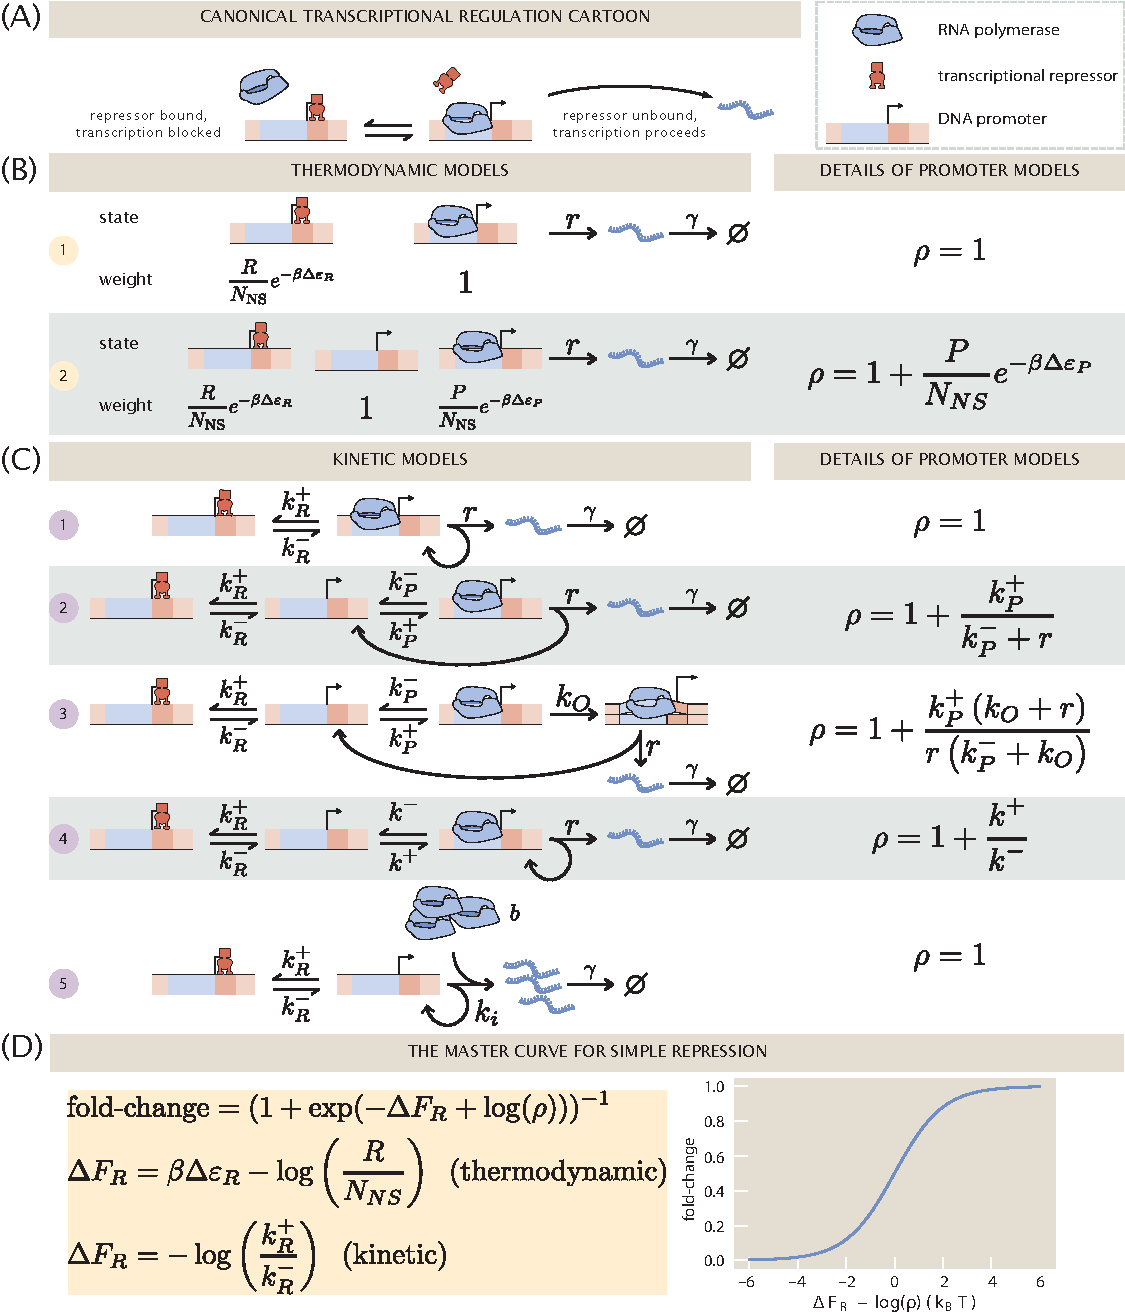
\includegraphics[width=\textwidth]{../../figures/main/fig01.pdf}
\caption{\textbf{An overview of the simple repression motif at the level of
means.} (A) Schematic of the qualitative biological picture of the simple
repression genetic architecture. (B) and (C) A variety of possible
mathematicized cartoons of simple repression, along with the effective parameter
$\rho$ which subsumes all regulatory details of the architecture that do not
directly involve the repressor. (B) Simple repression models from an equilibrium
perspective. (C) Equivalent models cast in chemical kinetics language. (D) The
``master curve'' to which all cartoons in (B) and (C) collapse.}
\label{fig1:means_cartoons}
\end{figure}

The logic of the remainder of the paper is as follows. In
section~\ref{section_02_means}, we show how both thermodynamic models
(Figure~\ref{fig1:means_cartoons}(B)) and kinetic models based upon the chemical
master equation (Figure~\ref{fig1:means_cartoons}(C)) all culminate in the same
underlying functional form for the fold-change in the average level of gene
expression with an effective free energy $\Delta F_R$ capturing the regulation
given by the transcription factor, and a term $\rho$ describing the level of
coarse-graining of the transcriptional events as shown in
Figure~\ref{fig1:means_cartoons}(D). Section~\ref{sec:beyond_means} goes beyond
an analysis of the mean level of gene expression by asking how the same models
presented in Figure~\ref{fig1:means_cartoons}(C) can be used to explore noise in
gene expression. To make contact with experiments, all of these models must make
a commitment to some numerical values for the key parameters found in each such
model. Therefore in Section~\ref{section_04_bayesian_inference} we explore the
use of Bayesian inference to establish these parameters and to rigorously answer
the question of how to discriminate between the different models.